\documentclass[11pt]{article}
\usepackage{amsmath, amssymb, graphicx, listings, color, geometry}
\geometry{margin=1in}
\usepackage{hyperref}
\usepackage{listings}
\usepackage{xcolor}

\definecolor{codegray}{gray}{0.45}
\definecolor{codeblue}{rgb}{0.26, 0.36, 0.75}
\definecolor{codegreen}{rgb}{0.0, 0.5, 0.0}
\definecolor{backgray}{rgb}{0.96, 0.96, 0.96}

\lstset{
  language=C++,
  backgroundcolor=\color{backgray},
  basicstyle=\ttfamily\small,
  keywordstyle=\color{codeblue}\bfseries,
  commentstyle=\color{codegray}\itshape,
  stringstyle=\color{codegreen},
  numberstyle=\tiny\color{gray},
  numbers=left,
  stepnumber=1,
  numbersep=8pt,
  tabsize=2,
  breaklines=true,
  breakatwhitespace=false,
  showspaces=false,
  showstringspaces=false,
  captionpos=b,
  frame=single,
  framerule=0.5pt,
  rulecolor=\color{black}
}

\title{Reed--Solomon (63,42) Decoder: Errors and Erasures with Detection}
\author{COM 5140 ECC Project 2 \\ \small{Spring 2025 -- 111511015 Pin-Jing Li}}
\date{}

\begin{document}

\maketitle

\section{Overview}
This project implements a Reed--Solomon decoder over \( \mathbb{F}_{64} \) for the (63,42) code used in Cinema Digital Sound. The decoder handles both errors and erasures, and enforces decoding bounds with explicit detection of uncorrectable cases.

We use a LSB-first polynomial representation:
\[
[a_0, a_1, \dots, a_n] \quad \text{represents} \quad a_0 + a_1x + \dots + a_nx^n
\]

\section{Decoder Architecture}
The decoder performs the following major steps:
\begin{enumerate}
    \item \textbf{Syndrome computation} \( S(x) \)
    \item \textbf{Erasure locator} \( \sigma_0(x) \)
    \item \textbf{Modified syndrome} \( S_0(x) = \sigma_0(x)S(x) \bmod x^R \)
    \item \textbf{Key equation} \( \sigma_1(x) S_0(x) \equiv \omega(x) \bmod x^R \) solved via the Extended Euclidean Algorithm
    \item \textbf{Error location} using roots of \( \sigma(x) = \sigma_0(x)\sigma_1(x) \)
    \item \textbf{Error evaluation} using Forney’s formula
    \item \textbf{Final validation} via post-correction syndrome check
\end{enumerate}

The decoder checks as in the handouts, 
\begin{itemize}
	\item \textbf{Condition (A):} \quad $\deg(\omega) \geq t_0 + \deg(\sigma_1)$ 
    \item \textbf{Condition (B):} \quad $\sigma_1(0) \neq 0$ 
    \item \textbf{Condition (C):} \quad $x^n - 1 \equiv 0 \mod \sigma(x)$ 
\end{itemize}
Some extra check trying to handle beyond-radius detections
\begin{itemize}
    \item \textbf{Locator-Root Agreement:} \quad $\deg(\sigma) = \text{\# of roots found}$ \\
    Validates Chien search: all claimed roots must be found. If not, decoding is beyond the radius.

    \item \textbf{Decoding Radius Budget:} \quad $t_0 + 2\hat{t}_1 \leq R$ \\
    If the detected error $\hat{t}_1=\deg(\sigma_1)$ is exceeding the budget, decoding is beyond the radius. 
	And also, if $t_0$ is directly exceeding the radius, the decoding will also be rejected here.

    % \item \textbf{Syndrome Recheck:} \quad $S(\text{corrected}) = 0$ \\
    % Final integrity check to confirm successful correction. If syndrome is nonzero after correction, decoding failed. 
\end{itemize}

\section{Alternative Key Equation Solver: Welch--Berlekamp Interpolation}
As an extension, we investigated using Welch--Berlekamp interpolation instead of the Euclidean algorithm.

The key equation
\[
\sigma_1(x) S_0(x) \equiv \omega(x) \bmod x^R
\]
can be interpreted as a rational function interpolation problem: finding polynomials \( \omega(x), \sigma_1(x) \) such that
\[
\frac{\omega(x)}{\sigma_1(x)} = S_0(x) \quad \text{at known evaluation points}
\]

This approach involves solving a linear system in the coefficients of \( \omega \) and \( \sigma_1 \), under degree constraints:
\[
\deg(\omega) < t_0 + \deg(\sigma_1), \quad \deg(\sigma_1) \leq \left\lfloor \frac{R - t_0}{2} \right\rfloor
\]

Welch--Berlekamp interpolation may be preferable in some hardware or symbolic applications, where rational interpolation is more natural than iterative polynomial division.

\begin{lstlisting}[language=C++, caption={an implementation of WB decoding}]
	pair<vector<int>, vector<int>> solve_key_wb(const vector<int>& s0, int e0) {
    int mu = (R - e0) / 2;
    int nu = (R + e0 + 1) / 2 - 1;

    int n_eqs = R;
    int n_unknowns = (mu + 1) + (nu + 1); 

    vector<vector<int>> A(n_eqs, vector<int>(n_unknowns, 0));
    vector<int> b(n_eqs, 0);

    for (int j = 0; j < R; ++j) {
        int x = EXP_TABLE[j + 1];
        int Sj = poly_eval(s0, x);  // S0(alpha^j)
        b[j] = Sj;

        int power = 1;
        for (int i = 0; i <= mu; ++i) {
            A[j][i] = gf_mul(Sj, power); // S0 * x^i
            power = gf_mul(power, x);
        }

        power = 1;
        for (int i = 0; i <= nu; ++i) {
            A[j][mu + 1 + i] = gf_sub(0, power); // -x^i for omega(x)
            power = gf_mul(power, x);
        }
    }

    // Solve the system A * [sigma1_coeffs | omega_coeffs]^T = b
    vector<int> sol;
    bool ok = solve_linear_system(A, b, sol); 

    if (!ok) throw RSDecodeError("WB solve failed");

    vector<int> sigma1(sol.begin(), sol.begin() + mu + 1);
    vector<int> omega(sol.begin() + mu + 1, sol.end());

    if (sigma1[0] == 0)
        throw RSDecodeError("WB failure: sigma1(0) = 0");

    int inv = gf_inv(sigma1[0]);
    for (int& c : sigma1) c = gf_mul(c, inv);
    for (int& c : omega) c = gf_mul(c, inv);

    return {sigma1, omega};
}

\end{lstlisting}
\section{Extension: Guruswami--Sudan List Decoding}



\subsection{Motivation}

In our current decoder, a failure occurs as soon as \( t_0 + 2t_1 > R = 21 \). But in many practical cases, even beyond that bound, the transmitted codeword may still be uniquely recoverable. The GS decoder leverages algebraic geometry to find \emph{all} polynomials \( f(x) \) of degree less than \( K \) that agree with a subset of the received points \( (x_i, y_i) \) with high enough multiplicity.

\subsection{Key Idea}

The GS decoder proceeds in two phases:

\begin{enumerate}
    \item \textbf{Interpolation:} Construct a nonzero bivariate polynomial \( Q(x, y) \in \mathbb{F}_q[x, y] \) such that:
    \[
    Q(x_i, y_i) = Q^{(0,1)}(x_i, y_i) = \cdots = Q^{(0,m_i-1)}(x_i, y_i) = 0
    \]
    for selected interpolation multiplicities \( m_i \), where \( (x_i, y_i) \) are the received (possibly corrupted) points.
    
    \item \textbf{Factorization:} Find all univariate polynomials \( f(x) \) such that \( Q(x, f(x)) = 0 \). These \( f(x) \) correspond to potential codewords.
\end{enumerate}

\subsection{Decoding Radius}

The GS algorithm can correct up to:
\[
t < n - \sqrt{n(K-1)}
\]
errors with high probability, where \( n = 63 \) and \( K = 42 \) in our case. This is significantly beyond the half-distance bound \( \left\lfloor \frac{d_{\min}-1}{2} \right\rfloor = 10 \).

\subsection{Benefits and Challenges}

GS decoding is deterministic, algebraic, and error-locating. It does not rely on soft information or probabilistic models. However, it is computationally more intensive due to bivariate interpolation and factorization, and may return multiple solutions.

In practical implementations, further ranking mechanisms (e.g., reliability scoring, CRC checks) are used to choose the most likely correct codeword from the list.

Did not have enough time to implement this before the deadline, hopefully can take a try throughout the summer.


\section{Testing Design}
We use a Python test generator that injects up to \( t_0 \) erasures and \( t_1 \) errors under the constraint \( t_0 + 2t_1 \leq 21 \), or beyond.

\begin{itemize}
    \item Input vectors are saved as \texttt{input.txt}
    \item Ground-truth messages saved as \texttt{answer.txt}
    \item Decoder output saved as \texttt{output.txt}, with \texttt{*} lines for failure
\end{itemize}
We run through all the cases that are within the decoding radius $t_0 + 2t_1 \leq R$ and comfirmed the correct decoding implementation.
\section{Detecting Behavior Far Beyond the Radius}
We fix \( t_0 + 2t_1 = 32 \), vary error-to-erasure ratio, and for each case we run through 10k signals

\begin{figure}[!h]
    \centering
	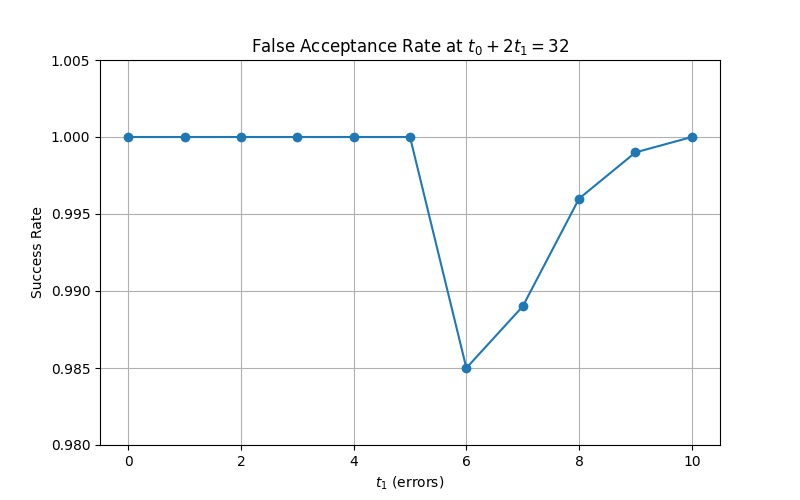
\includegraphics[width=0.8\textwidth]{fig/r32_rat.png}
    \caption{Testing the failure detection ability}
\end{figure}

\begin{itemize}
	\item test 1 has some false detection when $2t_1$ and $t_0$ has a closer value
    \item Perfect rejection near the boundary (all erasure / all error cases) 
    \item But rare false acceptances at extreme configurations, where the error pattern coincidentally satisfied all algebraic conditions.
\end{itemize}

\section{Decoder Behavior Just Beyond the Radius}
\label{sec:radius-edge}

While the classical decoding radius of a Reed--Solomon code is given by the bound \( t_0 + 2t_1 \leq R = N - K \), the behavior of algebraic decoders just beyond this radius exhibits subtle and non-monotonic phenomena. In this section, we examine this edge behavior both empirically and algebraically.

\subsection{Experimental Observations}
When only errors are presented, the decoder can almost always detect if the error was beyond radius. The following discussed the case when both erasure and errors presents. We fixed the number of injected errors to \( t_1 = 3 \), and varied the number of erasures \( t_0 \in \{16, \ldots, 21\} \), such that \( t_0 + 2t_1 > R \). Although all of these test cases technically exceed the decoder's guaranteed radius, we observed that the success or failure of the decoder varies dramatically with \( t_0 \). For instance, with \( t_1 = 3 \), the decoder’s ability to reject corrupted codewords showed a striking pattern:

\begin{figure}[!h]
    \centering
	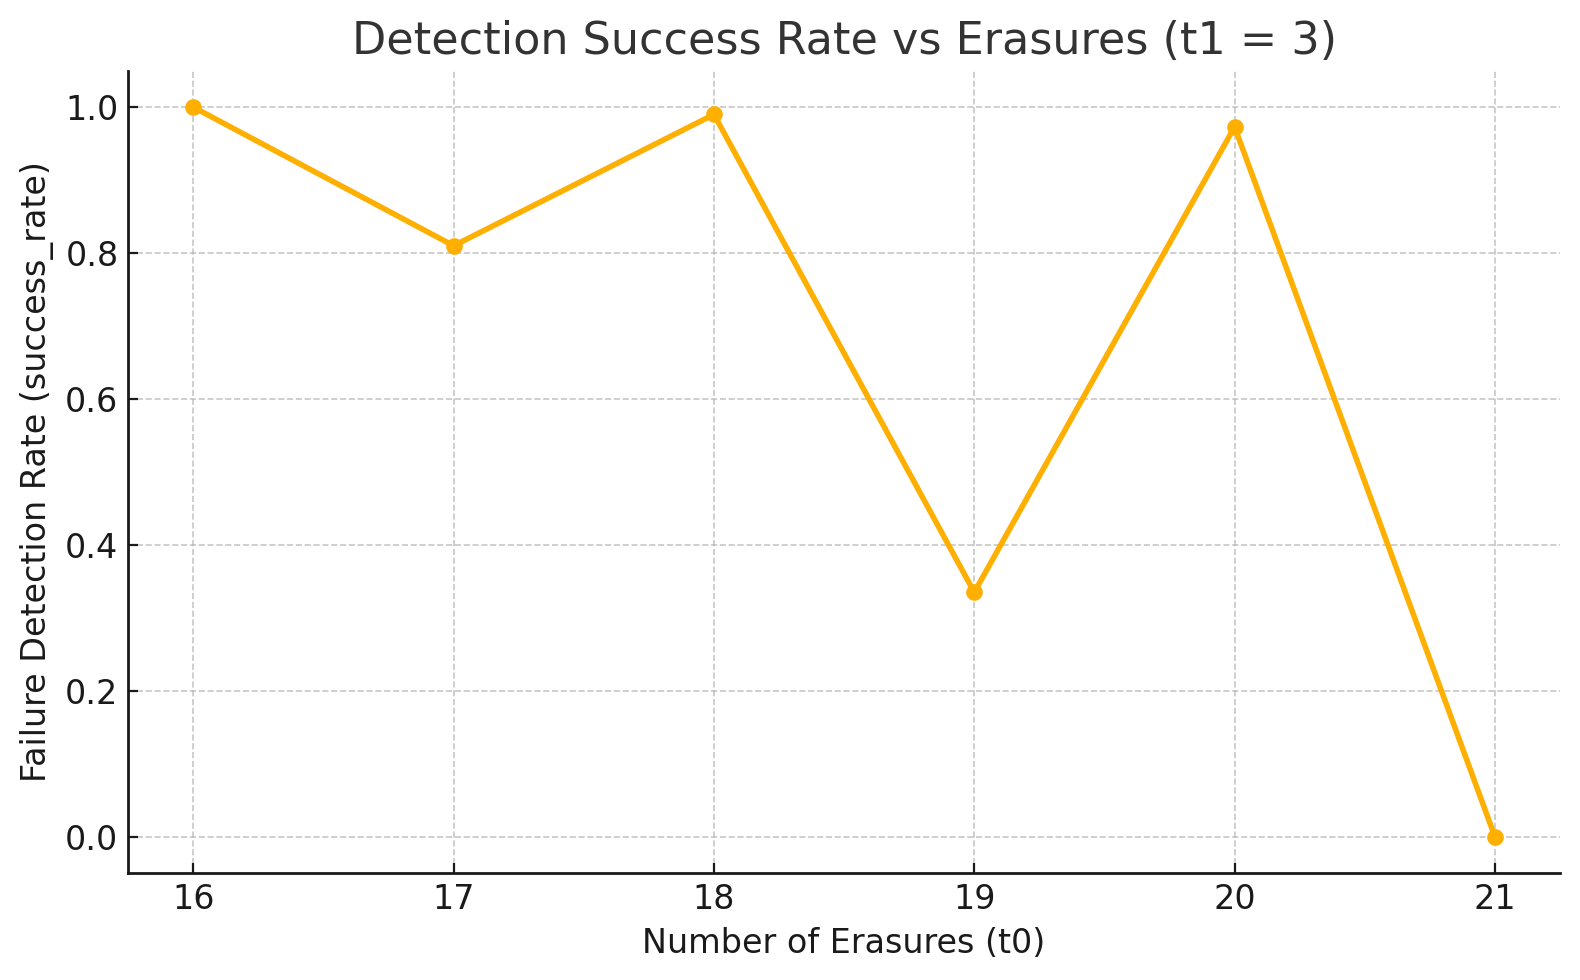
\includegraphics[width=0.8\textwidth]{fig/edge_test.png}
    \caption{Testing the failure detection ability just beyond the edge}
\end{figure}
Despite all cases exceeding the decoding bound, detection success is not monotonic in \( t_0 \). In particular, detection performance degrades drastically at \( t_0 = 19 \) and fails completely at \( t_0 = 21 \), even though the total decoding load is higher at \( t_0 = 20 \) and \( 21 \).

\subsection{Algebraic Interpretation}
This non-monotonicity arises from how the erasure locator polynomial \( \sigma_0(x) \) and the resulting modified syndrome polynomial \( S_0(x) = \sigma_0(x) \cdot S(x) \) affect the key equation:
\[
\sigma_1(x) \cdot S_0(x) \equiv \omega(x) \pmod{x^R}.
\]
As \( t_0 \) increases, the degree bound \( \mu = \left\lfloor \frac{R - t_0}{2} \right\rfloor \) imposed on the error locator \( \sigma_1(x) \) shrinks. When \( \mu = 0 \), the decoder is restricted to constant error locators, typically forcing \( \sigma_1(x) = 1 \). In this degenerate regime (e.g., \( t_0 = 21 \)), the decoder cannot model any error positions, and blindly trusts the message portion of the received word. Thus, even a single corrupted message symbol becomes undetectable.


\subsection{Implications}
These findings emphasize that the reliability of algebraic decoding just beyond the nominal radius is highly sensitive to the degree bounds in the key equation solver. While such decoders are mathematically correct, they may be semantically untrustworthy near the edge of their radius, particularly under full parity erasure. Implementations should therefore include structural checks on the syndrome and error evaluator polynomial, or impose additional constraints when decoding near \( t_0 \approx R \).


\section{Discussion}
These results confirm both the correctness and robustness of the decoder. The detection mechanism ensures that uncorrectable cases are rejected — even under randomized noise — unless they fall into pathological configurations.

Such false acceptances are theoretically known to occur when the erroneous received vector happens to lie within the decoding “ball” of some other codeword, even though it exceeds the designed radius. This behavior is consistent with the limitations of minimum distance decoding.


\appendix
\section*{Appendix: Decoder Source Code}
\lstset{basicstyle=\ttfamily\small, breaklines=true}
\lstinputlisting[language=C++]{commented_code.cpp}

\end{document}
